\documentclass[conference]{IEEEtran}
\IEEEoverridecommandlockouts
\usepackage{cite}
\usepackage{amsmath,amssymb,amsfonts}
\usepackage{algorithmic}
\usepackage{graphicx}
\usepackage{textcomp}
\usepackage{xcolor}
\usepackage{hyperref}
\def\BibTeX{{\rm B\kern-.05em{\sc i\kern-.025em b}\kern-.08em
    T\kern-.1667em\lower.7ex\hbox{E}\kern-.125emX}}
\begin{document}

\title{User-Driven COVID-19 Forecasting}

\author{\IEEEauthorblockN{Sebastian Häni}
\IEEEauthorblockA{\textit{School of Engineering} \\
\textit{Zurich University of Applied Sciences (ZHAW)}\\
Zurich, Switzerland \\
haeniseb@students.zhaw.ch}
}
\maketitle

\begin{abstract}
Many countries have introduced softly defined metric-based rules for entry and quarantine restrictions as a measure to slow down the spread of the COVID-19 virus. Citizens want to inform themselves where a country currently stands regarding these different metrics and desire a forecast to learn if the situation is improving or worsening. We describe a web platform that enables the average citizen to explore the data and visualize the exact metrics they are interested in and then let them personally create a forecasting model to their needs without requiring prior statistical knowledge. By providing highly interactive maps and charts we will give greater insights into the pandemic and its progress.
\end{abstract}

\begin{IEEEkeywords}
COVID-19; Statistical practice; Nonlinear regression; Time series
\end{IEEEkeywords}



\begin{figure*}[htbp]
\centerline{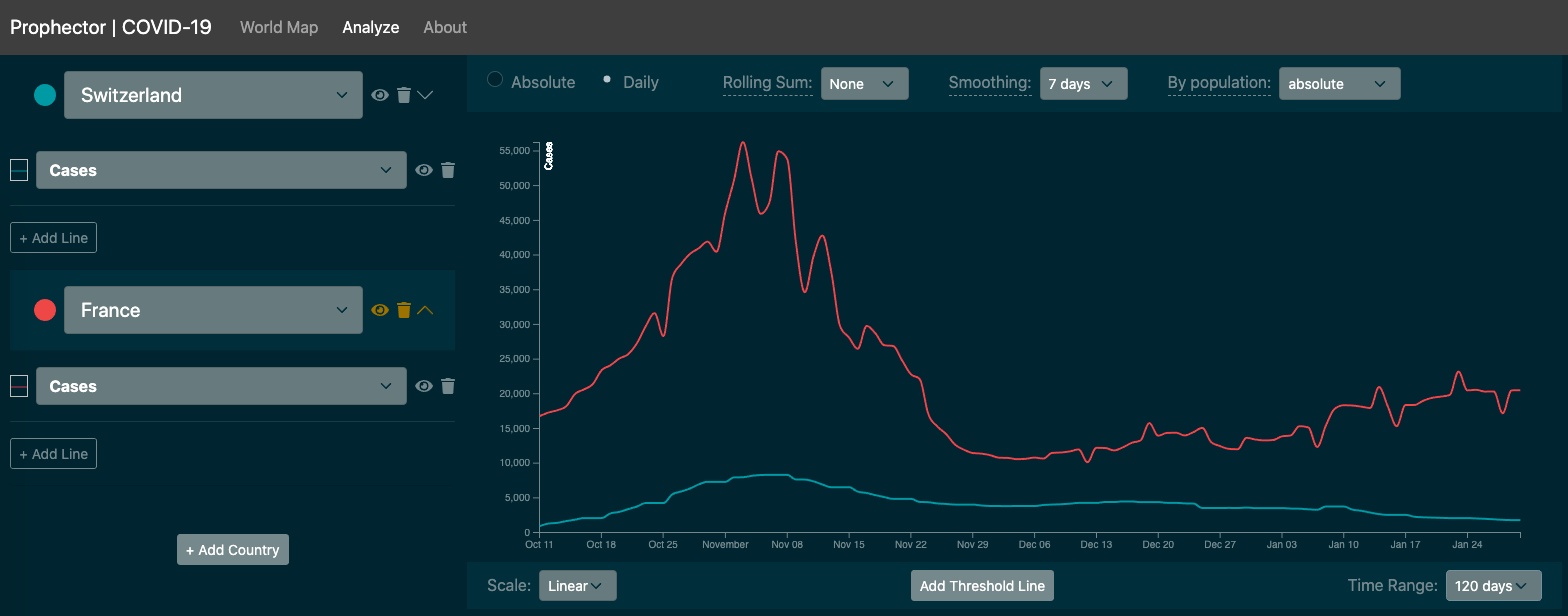
\includegraphics[scale=.328]{figs/screenshot-chart.png}}
\caption{The screenshot shows the chart analysis feature currently presenting time series data of daily cases in Switzerland and France, with a rolling mean with a window size of 7 days. The user is able to add, remove, or tweak the data selection on the left. Above the chart they can switch from absolute to daily data, change rolling sum, change rolling mean and normalization by population factors. Under the chart they can change the scale from linear to log, add a custom threshold line, and change the time frame to be shown from one to 90 days.}
\label{fig:screenshot-chart}
\end{figure*}


\section{Introduction}
The COVID-19 crisis challenges mankind in many ways and will not pass quickly, as many experts believe \cite{b6}. However, people have the desire to travel to other regions and countries within the limits of the regulations, whether for leisure or work purposes. Many countries have introduced softly defined metric-based rules for entry and quarantine restrictions. For example, the Swiss government has first defined a rule that the incidence in the last 14 days per 100,000 inhabitants of a region must be lower than 60, otherwise people returning from that area must be quarantined for 10 days. The government has since changed this rule to be relative to Switzerland's own metric. If a country has a metric 60 over the one of Switzerland, people entering from that area need to quarantine. Other countries have defined similar rules. Someone planning a vacation in the future would like to have access to the current and historic data aggregated according to these country-specific metrics, which are often not easily accessible. Additionally, they want to have a prediction of whether the country is likely to be on such a list in a few weeks.

It is trivial to find COVID-19 data \cite{b7}. That data is most often not interactively accessible for a consumer. They can download raw CSV files and write Python scripts to explore the data or they might look at charts generated by others. Many organizations and people are publishing their tables and charts online, but they don’t let one interact with them or only in a limited way.

\subsection{Combination Factor}

The combination factor is big and thus it's not possible to provide everything pre-generated. We could be interested in a combination of the following settings:

\begin{itemize}
    \item cases, tests, fatalities, vaccinations, test positivity rate
    \item country regions
    \item daily or absolute data
    \item linear or log scale
    \item rolling mean to provide curve smoothing with arbitrary window size (but most likely none, 7, 10, or 14 days)
    \item rolling sum with arbitrary window size to compute if a country-specific threshold has been surpassed or not (none, 7, 10, or 14 days)
    \item normalization by population factors (none, by 1,000,000, by 100,000, or by 10,000)
\end{itemize}

The possible amount of combinations is 244,480 assuming we have 191 countries or regions. Therefore, a practical solution lets the user define the settings they are interested in and generate the visualization on the fly. 


\subsection{Forecasting at Scale}

In the paper Forecasting at Scale \cite{b1}, Sean J. Taylor and Benjamin Letham described their solution to make the process of creating forecasts scalable in terms of limited human analyst capacity and automation. This is the approach we wanted to verify by making COVID-19 time series forecasts at scale.

With the amount of data produced and recorded by humans or machines it becomes difficult to create a forecasting model for each time series. The goal of having a super-model that can produce forecasts for any kind of time series data is very difficult to reach. We're focusing on a scalable approach that we can apply to produce reliable and high-quality forecasts for each time series separately. The challenge is the variety of time series and the lack of analysts that have expertise in their field and statistical training simultaneously. Completely automatic forecasting techniques can be hard to tune and are often inflexible to incorporate useful assumptions or heuristics. And domain experts are usually not trained in time series forecasting. This leads to a high demand for high-quality forecasts that outstrips the pace at which they can be produced \cite{b1}.

The type of scales talked about by Taylor and Letham are not computation or storage problems, as time series data usually does not have large disk requirements nor do forecasting models need a lot of computational power to be fitted today. According to the authors, scalable forecasting methods should be (1) suitable for many people, even if they have little training in forecasting, (2) suitable for a large variety of forecasting problems with idiosyncratic features, and (3) supporting efficient and automatic means of evaluation and comparing forecasts.

Once our COVID-19 time series is generated, we know the past and current state, but we would like to have a forecast of the next few days or weeks. Generating 244,480 forecasts daily is not feasible, even with Taylor and Letham's approach, in a cost effective manner, especially because most time series will likely never be looked at, and we don't know beforehand which ones those are. That's why we come to the same conclusion for forecasts as with visualizations: The user should be able to create a prediction themselves, while not requiring any statistics or programming know how. The prediction will also be displayed on their chart with \(yHat\) as well as lower and upper bounds that the fitted model generated in the backend.

This lets someone answer questions like "Can I travel to the Canary Islands in two weeks from now without having to go into quarantine upon return to my home country?".

\subsection{Justification}
A lot of solutions to the proposed problem exist already but there is still room for improvement.

Each item in this list points to an existing partial solution to the problems stated. For each item there's a justification what our solution will improve upon over the existing one.

\begin{itemize}
    \item The daily Tweets by the Federal Office of Public Health (FOPH) contain a lot of user generated statistics appended as replies.
    \begin{itemize}
        \item Our solution provides a way to explore many of the same data visualizations in an organized way with coherent design.
    \end{itemize}
    \item passportparty.ch contains blog posts with nice maps containing travel information that is unfortunately not updated daily, only contains Europe, and is not interactive.
    \begin{itemize}
        \item Our solution is capable of creating a similar geo map visualization but made interactive.
    \end{itemize}
    \item healthdata.org provides some projections which are not tweakable.
    \begin{itemize}
        \item Our solution is able to generate predictions on every type of time series (it is up to the user to decide if a prediction makes sense or not).
        \item Our solution allows a user to tweak the hyper-parameters and share them with others.
    \end{itemize}
\end{itemize}

\newpage
\section{Solution Design}

The system we built is running on the Amazon Web Services (AWS) cloud. AWS provides all the necessary building tools and infrastructure to make such a distributed computing system possible as well as cost-effective. Other cloud providers have a similar and perfectly suitable offering, and AWS was simply a choice of personal taste.

The result of the project consists of the following three parts A, B, and C and can be seen in figure \ref{fig:system}.

\subsection{Information Retrieval}
This component downloads data from a suitable source (or many sources) to get daily information. We implemented it using serverless functions written in TypeScript leveraging cost benefits of AWS Lambda.

\subsection{Web application}
The application features several interactive visualizations on different COVID-19 related time series with several interactive aggregations that can be applied by the user. 

Types of time series:

\begin{itemize}
    \item Cases
    \item Tests
    \item Fatalities
    \item Vaccinations
    \item Test Positivity Rate
\end{itemize}

Aggregations (and combinations thereof):
\begin{itemize}
    \item By country
    \item Absolute, by 100,000, by 1,000,000 inhabitants, …
    \item Moving average by 14 days, 7 days, …
    \item Moving sum by 14 days, 7 days, ...
\end{itemize}

To provide an easy entry into the application, the main visualization is a world map showing the daily cases, or any other user-chosen metric (with possible aggregations), of the current day or an aggregation of the past.

Furthermore, the application provides the user with predictions computed based on historic data with the aggregations applied. So, they can predict if they will likely have to quarantine themselves upon return from their visit abroad e.g., because the 14-day moving average per 100,000 inhabitants is likely to be above 60 at the planned end of their trip or whatever metrics their government has issued.

It is made clear that these predictions are to be read with care, and they are not legally binding. It may also happen quite often that a prediction is totally unusable.

We implemented the backend with Java and Springboot. The frontend implementation uses Angular, Mapbox, d3.js, and Bootstrap.


\subsection{Prediction Engine}

The backend of the web application provides a prediction engine. Time series prediction is not an easy task and can deem as almost impossible in many cases if the data is irregular. Nonetheless, COVID-19 data often has regular patterns that can be discovered by learning algorithms. Most time series have a weekly seasonality and a clear trend.

The paper "Forecasting at Scale" \cite{b1} explains ways how to scale up the process of creating forecasting models and making it even approachable to people with little or no knowledge in fields like statistics or data science. The authors have also provided many of the methods packaged in a Python and R library called Prophet.

Our solution provides the user a prediction with a click of a button for their selected time series and settings. Based on the result, the user can then decide to start tweaking the hyper-parameters of the initial model and create a new model. Typical hyper-parameters in a model are change points, holidays and seasonality, and smoothing parameters. After the user of the application is happy with their model, they can then publish their predictions and share it with others.

These user-defined forecasting models are then explorable by all users and shareable by a URL.

We implemented this part using Python and Facebook's Prophet.

\begin{figure*}
\centerline{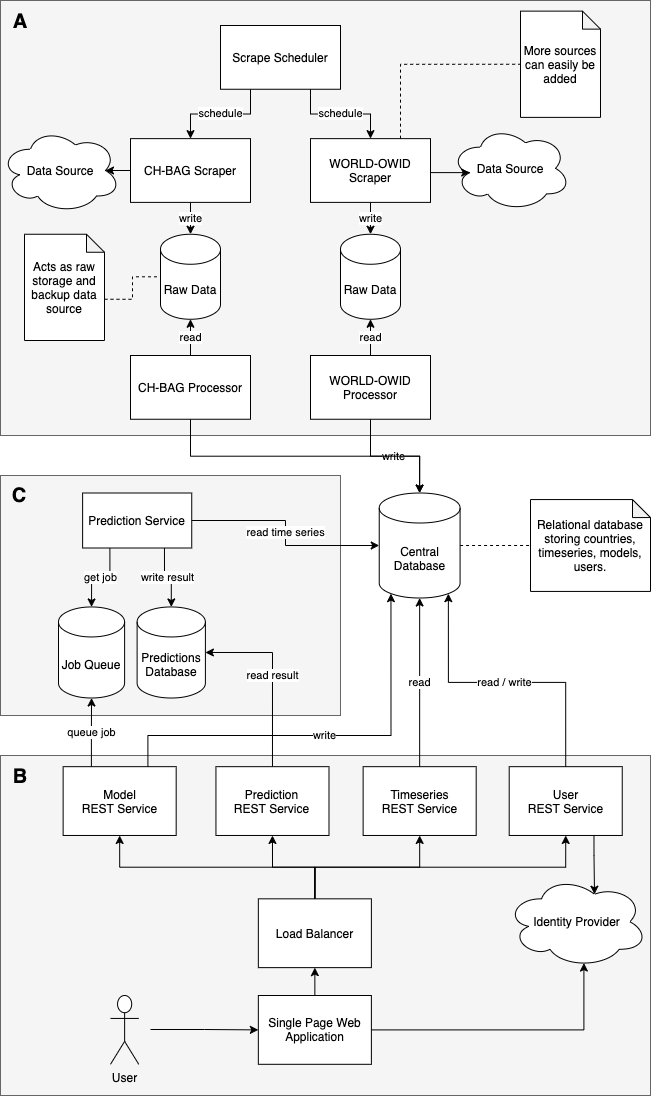
\includegraphics[scale=.5]{figs/system-diagram.png}}
\caption{Parts A, B, and C are grouped and consist each of several components. The central time series database is the way the three parts interact with the data. Part A: The information retrieval functions download the data from sources and import it into the database. Part B: The Web Application offers the end user a way to explore and interact with the data, as well as generate and retrieve predictions. Part C: The prediction engine listens for items in the job queue and executes them and stores the result back in a database, that the web application can then present to the user.}
\label{fig:system}
\end{figure*}


\section{Information Retrieval}

To visualize the time series to the user and create forecasts, we need to source the data first.

\subsection{Sources}

Daily COVID-19 data is fortunately quite easy to find in machine readable formats. Many governments publish their data daily, but the formats differ for each. We sourced the data of the Federal Office of Public Health\footnote{Link to FOPH API: \href{https://www.covid19.admin.ch/api/data/context}{https://www.covid19.admin.ch/api/data/context}} (FOPH) of the Swiss Confederation. This data contains country wide but also region-specific time series data with raw and aggregated metrics. We also looked at worldwide data from a single source and found Our World in Data\footnote{Link to OWID data: \href{https://ourworldindata.org/coronavirus-source-data}{https://ourworldindata.org/coronavirus-source-data}} (OWID) which publishes reliably daily data from almost every country. OWID has their own data pipelines sourcing their data from official sources to create one place to have all the data available in a coherent format. The FOPH later started publishing worldwide data as well, whereas they sourced it from OWID. The FOPH also uses OWID data to decide which country should be put on a risk list. So, since OWID seems to be a legit data source and even the FOPH trusts them, we decided to have OWID as our main data source but leave the architecture open for other sources to be integrated into the platform. In fact, the FOPH data is still sourced and present in the time series database, but not made available to the end user.

OWID is a good aggregator, as they do the heavy lifting for someone that wants easy access to raw data. For example, on November 30, OWID transitioned from the European Center for Disease Prevention and Control (ECDC) to Johns Hopkins University as our source for confirmed cases and deaths. This followed the ECDC’s announcement that they were switching from daily to weekly updates.

In contrast to OWID, the FOPH source also has hospitalization numbers, whereas OWID does not. We decided to not display hospitalization numbers for now, since they would only be available for Switzerland. And that would complicate the design of an easy-to-use user interface.

We found out that some countries report invalid data, such as Brazil and Tunisia, which report more COVID-19 cases than tests. It is not possible to have more cases with fewer tests. This obviously skews our map visualization for test positivity as we have positivity rates above 100\%.

\subsection{Data Processing}

We implement a scraper and a processor function for each source we want to integrate into our system. The scraper function downloads the files from the source by a tweaked schedule and places them in an AWS S3 bucket for easy retrieval. These raw files also serve as a backup to fully restore the time series database in case of a data loss by processing the data again. We can tune the schedule to download the data according to the sources' publishing schedule. For example, FOPH data is usually released between 13:00 and 14:00 CET/CEST, whereas OWID data is updated continuously.

The processor knows how to read the raw data, creates or updates the country entities with population numbers, if they don't exist yet, and populates the time series database by country and feature (i.e. cases, tests, deaths, vaccinations). It has to do a small amount of data correcting, as for some countries (e.g., tests in Germany) some data is not continuous, whereas it should be a strictly monotone series reporting the total for each day. In case we get a zero but had a larger value before that day, we fill it with the previous value. This error in the data happens, because OWID cannot infer the numbers in between publishings by the countries if they don't publish daily data. For our purposes this is fine, since we will show the daily data, which in this case will just have a spike once a week and the rest of the week it is zero in case somebody looks at the data without any smoothing.

The time series data is then stored in a central PostgreSQL database to make updating and querying the data straight forward. The choice of database does not matter much, since we are not dealing with a large amount of data. Our data is daily, per country and per series. The row count is below 100,000 and should never exceed 1,000,000. This amount can be handled quite easily by almost any database system. Other perfectly as good options would be relational database options such as MySQL, Microsoft SQL Server, or Oracle. NOSQL database options such as MongoDB would also work. We chose PostgreSQL because we were familiar with and because it can be run in a Docker container locally as well "as a service" in the public cloud.

\subsection{Serverless Functions}

The scraping and processing of COVID-19 data only has to be done once or a few times per day. Running a special server that has 100\% uptime handling that, is not cost effective. We decided to use serverless functions by AWS Lambda\footnote{\href{https://aws.amazon.com/lambda}{https://aws.amazon.com/lambda}}. These functions can be triggered by a schedule or by other events and only occur any cost when they are invoked, since they run on shared infrastructure ran by AWS. AWS has a free tier\footnote{\href{https://aws.amazon.com/free}{https://aws.amazon.com/free}} and offers 1 million lambda invocations per month free forever. This means, our information retrieval tool is free, since we do not exceed this limit by some margin.

\subsection{Database Migrations}

Our central database running with PostgreSQL has a schema. This schema needs to be managed and updated once new features are deployed. It is generally a good idea to have automated migrations that are executed by the system automatically by figuring out the outstanding schema migrations and applying them rather than a developer running SQL statements by hand. For that we also leveraged serverless functions and implemented a simple migration handler that updates the central database to a new schema. We decided to do this here, because the scraper and processors are responsible for the sourcing of data, and thus this is the place to also do database migrations. If we do the migrations driven by the web application for example, we will introduce a not straightforward flow of deployments, by first having to deploy the web application, that triggers a migration and only then redeploying the functions sourcing the data.


\begin{figure}
\centerline{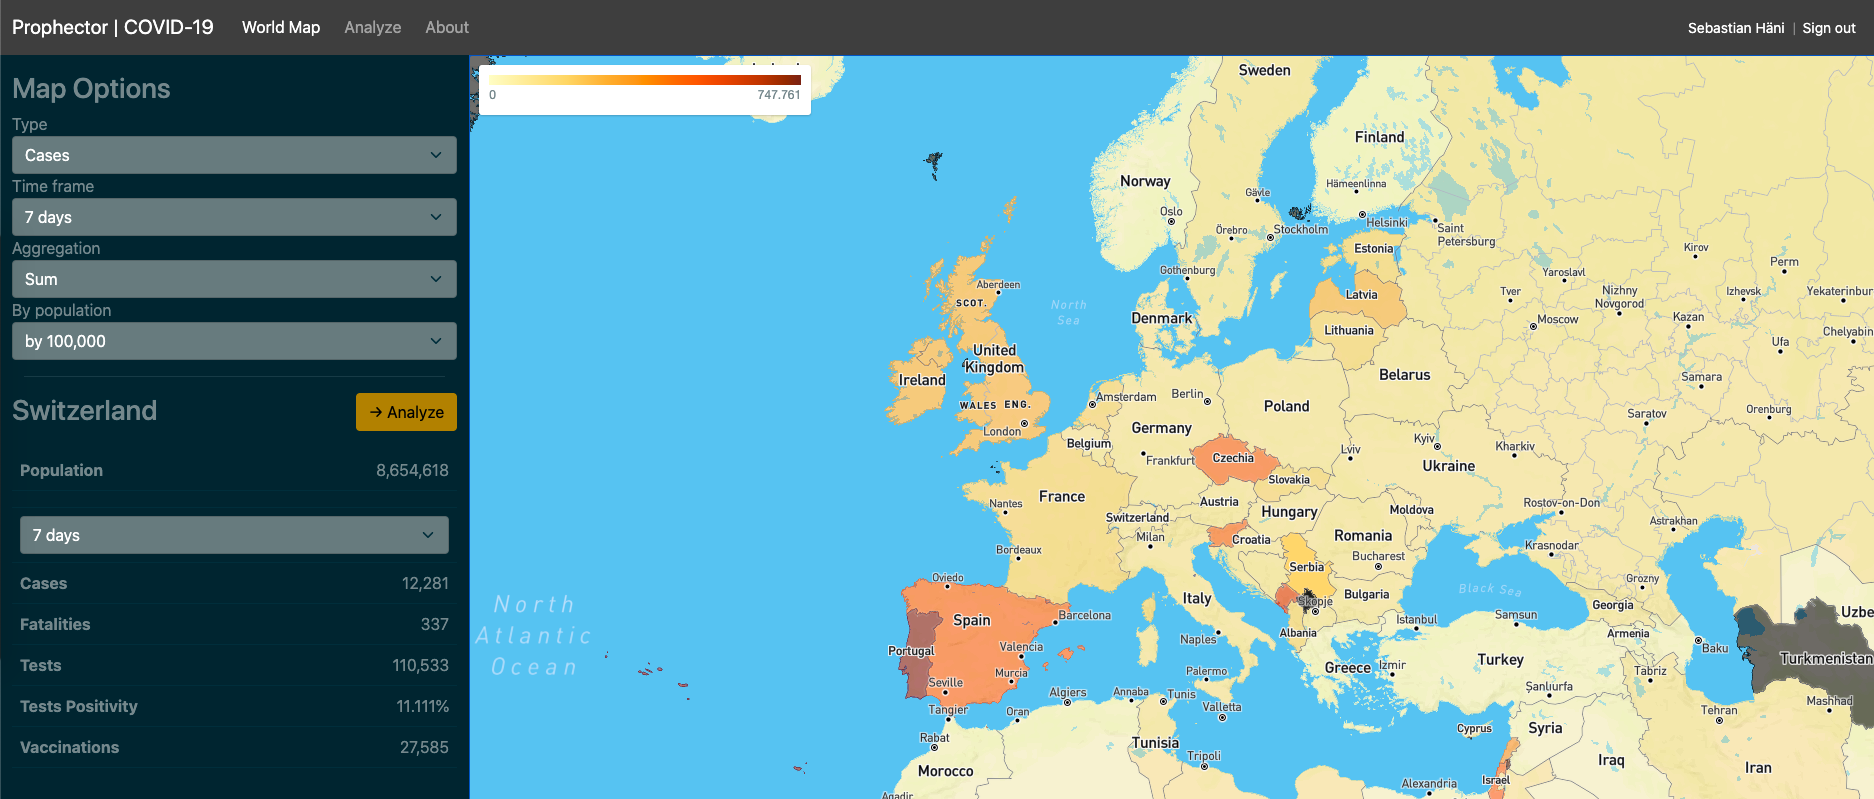
\includegraphics[scale=.135]{figs/screenshot-map.png}}
\caption{The screenshot shows the world map feature and the coloring of each country by cases summed in the last 7 days and normalized by the population factor. Currently Switzerland is selected.}
\label{fig:screenshot-map}
\end{figure}


\section{Visualizing COVID-19 data on a map}

The landing page of our web application is a world map visualizing the current state per country in a choropleth map as shown in figure \ref{fig:screenshot-map}. Each country receives a color on a scale of a statistical variable such as cases, tests, deaths, test positivity rate, or vaccinations within a time frame. The metric and aggregations can be changed individually by the user. This gives an overview and also an easy way to discover data as well as jump into a country's details.

With a map visualization come several challenges. The first one is the drawing of country polygons. Big and small countries should be discoverable while still being colored in according to our scale. The amount of polygon data is immense, and we didn't want to implement this ourselves. We used Mapbox\footnote{\href{https://www.mapbox.com}{https://www.mapbox.com}} which offers a JavaScript API to draw such maps. The maps are based on OpenStreetMap. The free tier of Mapbox includes 50,000 map loads per month.

The second challenge we encountered was preparing the data to visualize the map. Having just the raw time series in a database, we theoretically need to run aggregations for each country, which can involve querying thousands of data points. Since this data doesn't change over the course of minutes and rather over the course of a day, we added in-memory caching of the results in our backend. Once a new time window starts, the cache is invalidated and the first user accessing it, after it has been invalidated, has to wait roughly 10 seconds longer than the usual fast loading times, which was deemed acceptable by us (we actually pointed the health check to this URL, which means, it's likely that the health check triggers the refresh).

The third challenge is the color scale. Visualizing a map with all countries on a linear scale will skew visual inspections should there be an outlier in either direction. We decided to leave the scale linear as changing it to non-linear would also not be easy to recognize for a human, since a log scale is not easy to understand for a human. To generate a sequential color distribution over the linear scale, we used ColorBrewer\footnote{\href{https://colorbrewer2.org/\#type=sequential&scheme=YlOrRd&n=9}{https://colorbrewer2.org/\#type=sequential\&scheme=YlOrRd\&n=9}}. It contains several safe presets and directly gives a preview. The countries that have no data are colored in as black.

We added extra information to the map by providing helpful tooltips of the actual represented value as well as some additional information. Once the user clicks on a country, the country details appear, and the user is able to gather key metrics and can change the time frame for those interactively.

\section{Making COVID-19 time series interactive}

The main feature the user interacts with in our application is the chart analysis page as shown in figure \ref{fig:screenshot-chart}. The goal was to provide a powerful tool that can still be managed by an average user.


\subsection{User Features}
The user is able to select countries, and within countries show features such as cases, fatalities, tests, test positivity rate, and vaccinations. The different time series are automatically assigned a different color in case of countries or a different line dash pattern in case of features. Additionally, the user can choose the color they want to use for which country. For example, they might want to use red for Switzerland and blue for France. The different time series can be hidden or shown, without having to be removed.

The center chart shows the selected data and provides detailed information on hover. It displays the value of each series in a tooltip. We used d3.js to build this visualization.

The user can further change between absolute (totals) or daily rates. Should they decide to visualize absolute data, they might want to change the scale from linear to a log scale.

Furthermore, they can add a rolling mean or rolling sum with a given window size. To compare between countries, it is helpful to activate normalization by population. The user can choose between several population factors.

The visualizations also instantly update upon change of a setting. This is because the frontend makes exactly one call per country to the backend and retrieves the data for all features in the given time frame. This usually takes less than 200ms (measured by the client, which includes network latency)). From that point on, the frontend application computes all the transformations in the browser.

\subsection{Use Case Example}
A user might live in Switzerland. Switzerland has defined that if a country has 60 more cases in the last 14 days per 100,000 inhabitants than Switzerland, they will put it on the list of risk countries\footnote{\href{https://www.bag.admin.ch/bag/en/home/krankheiten/ausbrueche-epidemien-pandemien/aktuelle-ausbrueche-epidemien/novel-cov/empfehlungen-fuer-reisende/quarantaene-einreisende.html}{https://www.bag.admin.ch/bag/en/home/krankheiten/ausbrueche-epidemien-pandemien/aktuelle-ausbrueche-epidemien/novel-cov/empfehlungen-fuer-reisende/quarantaene-einreisende.html}}. 
To figure out if a given country should be on the list or vice versa, a user would go through the following steps in our application to create the visualization that gives them an answer:

\begin{itemize}
    \item Add Switzerland and another country to the chart. Select cases.
    \item Select daily data (default)
    \item Select rolling sum of 14 days
    \item Optionally select smoothing of 7 days to make the chart easier to read (this introduces a slight imperfection in the data)
    \item Select By Population of 100,000
    \item Select a shorter time frame to focus in on the recent weeks
\end{itemize}

The resulting chart can be seen in figure \ref{fig:che-vs-nld}.

\begin{figure}
\centerline{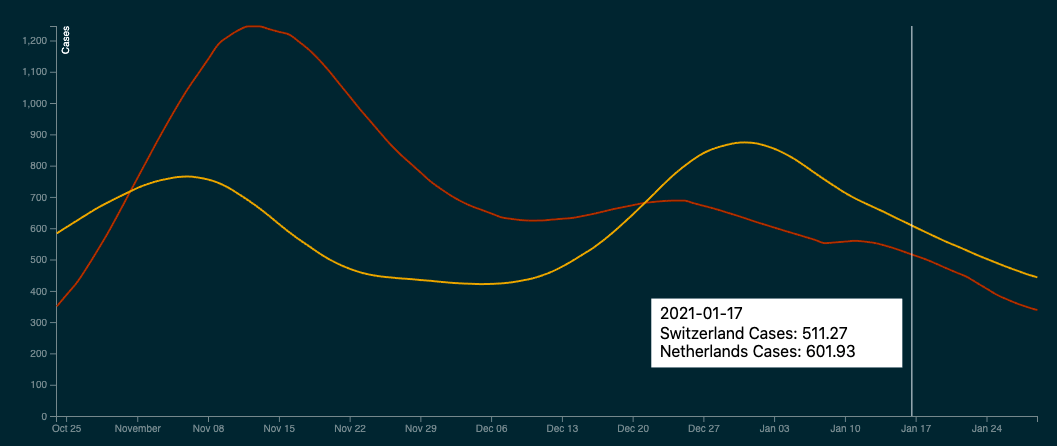
\includegraphics[scale=.23]{figs/che-vs-nld.png}}
\caption{The chart shows that the Netherlands has an incidence rate 90.66 higher than Switzerland on January 17, 2021. This should mean the Netherlands should be on the list of risk countries of Switzerland. It was not at the time of writing, which shows the government applies some leniency in their rules. It is probably not on the list because the trend is similar to the one of Switzerland and showing good signs. They also use an arbitrary cut-off date. A user interpreting this graph is able to read this information from it and can make their own conclusions which shows  the potency of our solution.}
\label{fig:che-vs-nld}
\end{figure}

\section{Forecasting COVID-19 time series}


\subsection{Data Selection}
We integrated the user interface for forecasting tightly with the chart analysis feature. They go hand in hand. The user visualizes the time series they are interested in. It follows that they also want to create predictions for exactly that time series. They can create a new model with a button and the data they previously selected is now the input data to train their model. They get to generate a forecast right away by using the default hyper parameters supplied by the system. Should they want to change the data (e.g., select a different time frame), they can easily update the chart and update their model and the forecast.

\subsection{Behind the scenes}
Once the user wants to fit their model to the data, the backend creates a job and adds it to a queue. The prediction engine takes the job and fits the model. It creates a forecast a third into the future of the original time frame length and writes the resulting prediction back into the database. This includes uncertainty intervals. We made the prediction horizon a third of the input data length, to (1) reduce the number of things users have to configure and (2) we don't want a user to be able to create forecasts too far into the future, as those will not be usable and potentially lead to the wrong conclusions.

The prediction engine is a small container running Python that can be scaled horizontally very well as it acts as a worker.

\subsection{Forecasting}

There are common time series features that we care about when creating a forecast. One are seasonal cycles, e.g., a weekly seasonality that shows recurring patterns throughout the weekdays or a yearly seasonality that might show a dip towards the end of the year for example. Another feature are trend changes over time. We might also notice effects of holidays events. And the last feature we can observe are outliers.

The authors of the paper Forecasting at Scale \cite{b1} explain the insufficiency of previous forecasting methods by taking an example time series that they recorded and tried fitting the data in an automated setting without changing the default parameters on these data. The referenced approaches were Autoregressive Integrate Moving Average (ARIMA) \cite{b2}, Exponential Smoothing \cite{b3}, and Trigonometric seasonality, Box-Cox transformation, Autoregressive Moving Average (ARMA) errors, Trend and Seasonal components (TBATS) \cite{b4} as well as an unreferenced naive approach using a random walk making constant predictions with a weekly seasonality.

The result was that these methods can be made to work, if one tweaks their parameters. Figuring out the parameter values can be tricky if the user is not trained in these models. For example, ARIMA has three main parameters (1) maximum order of differencing, (2) autoregressive components, and (3) moving average components. Without proper understanding of these parameters and their effects it is hard to find a good fit.

The authors created an R and Python library that implements the described methods of their paper and named it Prophet\footnote{\href{https://facebook.github.io/prophet/}{https://facebook.github.io/prophet/}}.

\subsection{The Prophet Forecasting Model}

We know the features of a time series. We can model this as separate components that we additively combine to a prediction model. We add the trend \(g(t)\) modeling nonperiodic changes, the seasonality \(s(t)\) modeling the periodic changes, the holidays and events \(h(t)\) modeling single data point effects which are potentially irregular, and the error term \(\epsilon_t\) that is assumed to be normally distributed.


\begin{equation}
    y(t)=g(t)+s(t)+h(t)+\epsilon_t
    \label{eq:fullTrendModel}
\end{equation}


The advantages of this model are 

\begin{itemize}
    \item computationally simple, making fitting it to data very fast
    \item cognitively simple, making it easily interpretable by human analysts
    \item adding new components is easy since we're using addition and no normalization factors need to be introduced
\end{itemize}


The addition aspect of the model however means that we cannot model a trend change that amplifies the effects of the seasonality component as they are assumed to be independent. The authors later made their software Prophet capable of producing forecasts with multiplicative seasonality as well, after the publishing of the paper. We allow users to select which seasonality mode they want to use to train their model. If the magnitude of seasonality effects grows with the time series itself, it could be interesting for the user to use multiplicative seasonality. 

\textbf{Trend:} The mathematical expression to compute the nonlinear, saturating growth trend in its most basic form is the standard trend formula with \(C\) as the carrying capacity, \(k\) as the growth rate, and \(m\) as an offset parameter.

\begin{equation}
    g(t)=\dfrac{C}{1+exp(-k(t-m))}
    \label{eq:simpleTrendModel}
\end{equation}

This gives us a formula that supports a static carrying capacity and static growth rate. In the real world, capacity and growth rate are often not static and need to be dynamic. We can replace the carrying capacity \(C\) with an analyst-specified dynamic capacity function based on time \(C(t)\). The growth rate \(k\) can be replaced with a vector \(a\) that contains the manually specified change points with the respective growth rate of that time interval. This gives us the new formula.

\begin{equation}
    g(t)=\dfrac{C(t)}{1+exp(-(k+\boldsymbol{a}(t)\boldsymbol{^\tau}\boldsymbol{\delta})(t-(m+\boldsymbol{a}(t)\boldsymbol{^\tau}\boldsymbol{\gamma})}
    \label{eq:prophetTrendModel}
\end{equation}

When simplified, it will give us a linear trend with change points by removing the carrying capacity, and a constant growth replaced by rate adjustments.
By default, Prophet uses this piecewise linear model to fit the trend, which is does not have capacity parameters. That would be fine to use for growing trends, but since many of our time series have a decreasing trend towards zero, no cap and no floor means the model will start to predict numbers below zero. Therefore, we chose a logistic growth, as per equation \ref{eq:prophetTrendModel}. We define the floor of the trend to be 0. The cap is a multiple of 10 of the maxima in the existing data. We would like to specify an infinite cap, but this causes overflow issues in the implementation of Prophet.


The uncertainty of this model is computed by using it generatively, after having inferred the model parameters, to forecast the future, while assuming the rate of change points is going to have a similar average cadence. We can repeat the generation while sampling the model parameters from a Laplace distribution and create an uncertainty region.

The change points can be generated automatically, or a user can set them specifically. They model at what points the trend will change. If we introduce too many change points, we are not going to fit a trend correctly that lasts longer than the time frame between two change points. If we had too few, the model might result in a high error term because it does not have enough flexibility. Reducing the amount of change points is a regularization method.

The change points can be found automatically by putting initial change points uniformly onto the time series data for the first 90\% of data. The authors recommend 25 initial change points. If we would spread the change points on 100\%, the model will not have enough capacity to fit an emerging trend that we are most often interested in, in a forecast. Once we have the initial change points, we put a sparse prior on these change points and compute each point's magnitude. The prior variable is a hyper-parameter that also acts as regularization. Once we have the magnitudes computed we can discard change points with a low value and keep the remaining ones.

\textbf{Seasonality:} Since seasonality in the real world is mostly a composition and does not have a fixed window in which it repeats, it can be flexibly modeled using Fourier series. If we have different components for different periodic effects, such as yearly, holiday or weekday components, we can create an additive model based on that. A standard Fourier series can approximate arbitrary smooth seasonal effects with the following formula, where \(P\) is the period.

\begin{equation}
    s(t)=\sum\limits_{n=1}^N (a_n cos(\frac{2\pi nt}{P})+(b_n sin(\dfrac{2\pi nt}{P})))
    \label{eq:prophetSeasonality}
\end{equation}

The variables \(a_n\) and \(b_n\) are the ones fitted to the data. In the seasonality model, we have to tweak the number of Fourier components \(N\) we want to define. Specifying too few will not allow the model to adequately approximate the seasonality and specifying a value too high will result in overfitting. The authors recommend \(N\) to be 10 for yearly and 3 for weekly seasonalities.


\textbf{Holiday Effects:} Holiday effects or events are somewhat predictable shocks to the time series. They are often appearing aperiodic and are assumed to be independent. A user has to specify the event dates manually. The model will be able to fit a corresponding change of the event to the forecast.

A holiday can be attributed to a single date in the year or a consecutive window of days. For example, Christmas can be considered a two-day holiday.

 We allow our users to add the holiday calendar of the country selected to the model fitting process.

\subsection{Model Fitting}

\begin{figure}
\centerline{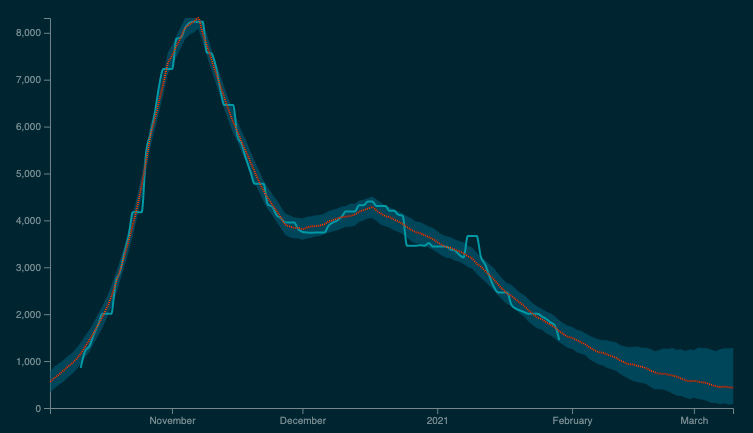
\includegraphics[scale=.328]{figs/screenshot-prediction.png}}
\caption{The visualization generated after creating a prediction model. We can see the prediction knows about a saturating minimum of zero and approximates this number slowly when predicting into the future. Blue line: the actual time series used to fit the model. Red line: \(yHat\). Blue area: uncertainty interval.}
\label{fig:screenshot-prediction}
\end{figure}

The model can then be fitted with Stan \cite{b5} specifying the distributions to sample from for the different parameters. The user choosing the prior variables is supported by our boundary visualizations that show the effects of the latest changes to their model as seen in Figure \ref{fig:screenshot-prediction}.

\subsection{Analyst-in-the-Loop Modeling}

The user, our analyst, is in the loop while modeling and can define a set of parameters to introduce their knowledge to receive a reliable and high-quality model.

\begin{itemize}
    \item \textbf{Change points:} Known dates of change points, such as dates of governments putting measures into place, can be directly specified.
    \item \textbf{Holidays and seasonality:} Users can enable country holidays for the model to learn these effects.
    \item \textbf{Smoothing parameters:} By adjusting the smoothing parameter a user can select from within a range of more global or locally smooth models. The seasonality and holiday smoothing parameters allow the user to tell the model how much of the historical seasonal variation is expected in the future.
\end{itemize}

We don't provide component charts to the users yet, where trend, seasonality, and holiday effects can be inspected individually. This would be a helpful future improvement to understand what effect the latest parameter change yielded in exactly. 

The full list of hyper parameters can be seen in table \ref{tab:hyper-params}.

\begin{table*}
  \caption{Hyper Parameter List}
  \centering
  \begin{tabular}{|p{3.5cm}||p{1.6cm}|p{1.6cm}|p{9.6cm}|} % must sum to 16.3cm
     \hline
     Parameter & Default Value & Customizable & Comments\\
     \hline
     \hline
     $growth$                    & logistic         & no  & The other option $linear$ does not respect caps or floors, and thus would produce invalid forecasts. We specify a cap of \(max(df) * 10\) to ensure we have enough head room and not run into integer overflow problems. \\
     \hline
     $changepoints$              & auto detection & yes & This is a list of customizable change points, if the user wants to define it themselves. If this is empty, we use the setting of $n\_changepoints$ to auto detect change points. \\
     \hline
     $n\_changepoints$           & 25             & yes & The number of change points of 25, should likely fit COVID-19 data. If the user selects a short time frame or want to apply regularization, they might want to reduce this number. \\
     \hline
     $changepoint\_range$        & 0.9            & yes & The model will use this percentage range to detect change points and will not place any in the remaining data. E.g., a trend change in the last 10\% will likely produce a bad forecast. We increased this number from 0.8 which was recommended by the authors of Prophet to allow the model to cope with all the measures put into place against COVID-19 and also produce slightly wider uncertainty bounds, which does not lead users into taking the prediction too seriously.  \\
     \hline
     $yearly\_seasonality$       & off            & no  & Our data barely covers a year, and certainly we need to wait several years until we could try and find yearly seasonality. For that to work, the virus must also stick around quite a while, which we all hope it will not. \\
     \hline
     $weekly\_seasonality$       & auto           & no  & We know COVID-19 data has a pretty strong weekly seasonality. So, we leave this on auto. \\
     \hline
     $daily\_seasonality$        & off            & no  & We don't have sub-daily data, so we turn it off. \\
     \hline
     $holidays$                  & off            & yes & The user is able to add the holidays of the country, read from the Python holidays library, to the model if they wish to. The effects are only marginal and do not apply yet, because holidays usually have a yearly interval, and we need more data to fully make use of this. Nonetheless it is interesting to see that the model can extract holiday effect on past data, even it cannot apply it to forecasts. \\
     \hline
     $seasonality\_mode$         & additive       & yes & This is only relevant, if the user creates forecasts without smoothing. They can change the setting to multiplicative. \\
     \hline
     $seasonality\_prior\_scale$ & 10             & yes & This parameter controls the flexibility of the seasonality. \\
     \hline
     $holidays\_prior\_scale$    & 10             & yes & This controls flexibility to fit holiday effects. \\
     \hline
     $changepoint\_prior\_scale$ & 0.5            & yes & This is probably the most impactful parameter. It determines the flexibility of the trend, and in particular how much the trend changes at the trend change points. The authors of Prophet recommend a default value of 0.05, but we change this default to be 0.25 for our use case. The trend changes in the past have been pretty strong, as measures put into place actually have their desired effect and turn around curves 90°. This fact also reveals that our predictions will not be "that" good. \\
     \hline
     $mcmc\_samples$             & off            & no  & We disable Monte Carlo sampling which can be used to not only get uncertainty in trend, but also the uncertainty in seasonality. Most of the time we are not interested in seasonal effects when creating forecasts for COVID-19 data. It also uses a lot more compute resources than Maximum a posteriori (MAP) estimation (which we use instead). \\
     \hline
     $interval\_width$           & 0.8            & no  & This is the percentage width of the uncertainty interval. We decided that this parameter is not customizable, since it doesn't change the prediction, only how it is visualized. This parameter makes sense if you use Prophet to do anomaly detection, whereas you can tune it to give you more or less anomalies according to feedback. \\
     \hline
  \end{tabular}
  \label{tab:hyper-params}
\end{table*}

\subsection{User Authentication}
To create a forecast, a user needs to be logged in to our system. They can use social identity providers such as Google or GitHub. This way they don't need to create a new account with a new password to remember.

We require users to be authenticated, so we can associate a generated prediction to a person. This lets users find their models again easily, even when logged in on a different device, and solves the question of who can edit an existing model, it's the owner of the model. It also allows us to display the name of the creator next to a prediction, should a prediction model be published and made discoverable. By making clear that a prediction has been created by another user, we implicitly transmit a message to users discovering this prediction that this is not machine generated and that a person created this (albeit with a lot of help from a machine). This automatically makes users think different about a prediction. They will know that humans are imperfect (especially on the Internet) and produce results that might be inaccurate or unusable. If we would provide predictions to all users by the system, they might fall into a false sense of certainty, that this forecast must be true, and might make conclusions that are dangerous for themselves or others. 

\section{Evaluating Models}

The user can optimize a model well given enough time. To facilitate comparison between models of different users, our system can rank created models in order of the error term. We call this the score of the model, the lower the score the better. This score is shown in the UI and gives a user a goal, to achieve a better score than a competing model.

\subsection{Simulated Historical Forecasts}
The metric used to compare models is the Mean Absolute Percentage Error (MAPE) over a number of forecasts produced with different prediction horizons.

Time series data points are inherently dependent on previous points. This is making it hard to use traditional methods. The method proposed in ``Forecasting at Scale`` \cite{b1} is Simulated Historical Forecasts (SHFs), that produce \(K\) forecasts at various cutoff points in the history. The generally used number of points is a forecast every \(H/2\) periods. This allows the model error term to be measured in MAPE which can be compared to other models. 

Time series data usually encompasses a lot of data points and running SHFs with the maximum number of periods would not be feasible as the model needs to be refitted as many times as there are points in the data. With SHFs, the simulation count is significantly reduced, and the computation can run independent in several processes or separate machines.


\subsection{Identifying Large Forecast Errors}

Using SHFs we can find common error patterns when producing forecasts. The main errors to look at are as follows:

\begin{itemize}
    \item A large error compared to the baselines usually means the model is misspecified. The analysts most likely need to change the trend and / or seasonality components.
    \item If we discover a large error on all methods on a particular date, we have found suggestive outliers. The analyst can be asked to confirm to remove these outliers by a supporting system.
    \item If the error sharply increases from one cutoff to the next, the analyst could introduce a change point there to fix the error.
\end{itemize}

\subsection{Limiting}
In our setting we decided to limit the number of simulated forecasts to \(K=5\) to save compute cost and to improve the responsiveness of our system for the user. This is still enough to produce a relevant score but is of course subject to statistical fluctuations. In our findings, these fluctuations are present even with higher numbers of forecasts, and only disappear with a significant amount, taking tens of minutes to compute, which is not feasible for us, as we want to produce evaluations in less than a minute.

We validate the model with a 14 day horizon \(H\) using SHFs, as we decided 14 days is a relevant horizon for COVID-19 models. As government measurements are put into place, the data is irregular seen over longer periods, and thus predicting too far in the future is meaningless. To limit the simulated forecast count, we first set the initial data point count to be \(I = H  * 3\) and then compute the period, which gives us a period independent of the length of the data set that will result in 5 simulated forecasts.

\begin{equation}
    P=\dfrac{df[-1]-df[0]-H-I}{5}
    \label{eq:shfPeriods}
\end{equation}

We don't present the full cross validation error term per horizon but only the final one with a 14 day horizon. This is a single number which can easily be used by users to compare their results and to sort prediction lists according to this score.

In the future we want to present users comparisons with baseline models such as a model using the last value, or a sample mean.


\section{Scaling and cost factors}

The system as described in figure \ref{fig:system} is designed to be easily scaled. By using the minimal amount of compute, storage, and networking, the system can be operated on a public cloud such as AWS quite cost efficiently. Should there be a rise in users we can identify scaling needs by built-in monitoring solutions or even define auto-scaling strategies to automatically scale with the users using the system, to always only use what we actually need and therefore only get billed for what we used. 

\subsection{Scraping}
The scraping functions, which use a serverless infrastructure, store data in S3 buckets on AWS, which have an unlimited storage. Both functions and S3 storage can be scaled very well.

\subsection{Central Database}
We used one central physical database to store countries, time series, models, predictions, users, and jobs to save costs, by not having to run multiple database instances. Should there be a need, we could separate the database into separate physical databases storing different entities. We would likely extract country and time series data into a separate one because the only parts of our system writing into that database are the data processing functions. The web backend and the prediction engine read from it, making it suitable for read-only scaling.

We could further extract predictions made by the prediction engine into its own database, as only the prediction engine writes data, and the web backend reads data.

\subsection{Web Backend}
The web backend is a Java container running a Springboot application, which needs quite a lot of memory just to start up. The smallest instance types of AWS do not have enough memory, which is why we could not make use of the AWS Free Tier to run the backend and instead used a VM that has 2 GB of memory. The one instance should however be capable of handling a lot of load, since there are no real computationally heavy operations to be performed by it. The backend merely handles authentication, querying data from the database and queuing prediction jobs.

\subsection{Prediction Engine}
The prediction engine uses a worker pattern and is perfectly suited to be scaled to more instances. Each worker fetches pending jobs from the queue, and once they start processing the data, they make an optimistic write to the database that it starts working on the job, and if that fails, it skips the job, because apparently some other worker already grabbed it in the meantime.


\section{Conclusion}

The entry barrier to investigate COVID-19 time series has been significantly lowered by our solution, as it is providing users with many options to choose how they want to inspect the data in a way that is relevant to them, without having to produce each possible combination of settings beforehand for them. Our system is capable of ingesting the data autonomously from different sources such as ``Our World in Data`` and ``FOPH`` and making it available to everyone with Internet access.

We showed how such a system can be engineered in a scalable and cost-effective way on public cloud infrastructure while still performing fast executing user actions. Our application also showcases how a user interface can be designed to accommodate complex use cases such as inspecting time series interactively, adding comparison data, creating prediction models and visualizing such predictions while not overloading the user or confusing them.

With our solution it is also possible to let users compete creating better models and sharing them by URL because they all have a score attached. Those scores are additional information which can be used to quickly find a suitable model, while still allowing everyone, even not logged in users, to view those predictions.

The solution has room for improvement regarding the aforementioned score, which is a number that can be misleading because it has been produced with minimal compute and it is not the full result of the validation either. An improvement would be to store the complete result and show the SHF graph to the users, when they select a prediction, which allows for better judging of the model performance.

Additionally, it would be great if users could even compare regions that are smaller than a country. E.g., a user might want to compare the regions of their own country. This has proven difficult to implement, (1) it is not easy to get data for all possible regions worldwide as we would need to source our data from specific governments from almost every country, and (2) adding another hierarchy layer to the UI where the user can select a country, or a sub-region will complicate the UI.

Some COVID-19 series contain outliers, e.g., some countries had mass testing of the population, which skews testing numbers massively for a few days. Such outliers should probably be removed manually by the user creating a forecast. Our solution currently does not provide the possibility to remove such outliers. A future improvement would be to let users select a date or range of dates to be removed from the data. Prophet can easily handle missing data and would not have a problem.

We are sure our solution is appealing to many users and is providing value to them.

\begin{thebibliography}{00}
\bibitem{b6} Anderson, Roy M and Heesterbeek, Hans and Klinkenberg, Don and Hollingsworth, T D{\'e}irdre (2020), ``How will country-based mitigation measures influence the course of the COVID-19 epidemic\text{?}``, The lancet, 395, 931--934
\bibitem{b7} Roser, Max and Ritchie, Hannah and Ortiz-Ospina, Esteban and Hasell, Joe (2020), ``Coronavirus pandemic (COVID-19)``, Our world in data
\bibitem{b1} Sean J. Taylor \& Benjamin Letham (2018), ``Forecasting at Scale``, The American Statistician, 72:1, 37-45.
\bibitem{b2} Hyndman, R. J., Khandakar, Y., et al. (2007), ``Automatic Time Series for Forecasting: The Forecast Package for R,`` number 6/07, Monash University, Department of Econometrics and Business Statistics.
\bibitem{b3} Hyndman, R. J., Koehler, A. B., Snyder, R. D., and Grose, S. (2002), ``A State Space Framework for Automatic Forecasting Using Exponential Smoothing Methods,`` International Journal of Forecasting, 18, 439–454.
\bibitem{b4} De Livera, A. M., Hyndman, R. J., and Snyder, R. D. (2011), “A State Space
Framework for Automatic Forecasting Using Exponential Smoothing Methods,” Journal of the American Statistical Association, 106, 1513–1527.
\bibitem{b5} Carpenter, B., Gelman, A., Hoffman, M., Lee, D., Goodrich, B., Betancourt, M., Brubaker, M. A., Guo, J., Li, P., and Riddell, A. (2017), “Stan: A Probabilistic Programming Language,” Journal of Statistical Software, 76, 1–32.
\end{thebibliography}
\vspace{12pt}

\end{document}
